\documentclass[12pt,oneside,a4paper]{article}

\usepackage[margin=2cm]{geometry}
\usepackage[utf8]{inputenc}

\usepackage{graphicx}
\usepackage{titling}
\usepackage{float}
\usepackage{indentfirst}
\usepackage{setspace}
\usepackage{hyperref}
\usepackage{bookmark}

\graphicspath{ {../images/} }
\hypersetup{
  colorlinks=true,
  linkcolor=blue
}

\pretitle{%
  \vspace{4cm}
  \begin{center}
   \LARGE
   
\includegraphics[scale=0.1]{logo-usth-pa1-01.png}\\[\bigskipamount]
}
\posttitle{\end{center}\vspace{4cm}}

\title{
  {\Large \textbf{Advanced Programming with Python}\\}
  {\Large \textbf{Mobile Phone Store Information System Manager}\\}
\bigskip
  {\Large \textbf{Project Report}\\}
}

\author{
  Group 17
  \vspace{2cm}
}

\date{June 2021}

\begin{document}

\begin{titlepage}
  \maketitle
  \thispagestyle{empty}
\end{titlepage}

\tableofcontents

\addcontentsline{toc}{section}{List of figures}
\listoffigures

\newpage

\section{Introduction}
\subsection{Topic}
Mobile Phone Shop Information System Manager

\subsection{Application overview}
\begin{itemize}
  \item Written in Python and Tkinter (for user interface)
  \item Has fixed size, therefore should be used in full screen
  \item It is a minimal demo
\end{itemize}

\subsection{Why people need to use our project}
\begin{itemize}
  \item They might find the project interesting and give it a try
  \item They might need to manage small mobile phone store
  \item It provides a good minimal base for developing a working management product
\end{itemize}

\subsection{Responsibilities}
\begin{itemize}
  \item (BI10-063) Do Quang Hieu: Leader, programmer
  \item (BI10-112) Nguyen Hoang Minh: Database designer, programmer, data collector
  \item (BI10-097) Nguyen Khanh Lien: Slides and data collector
  \item (BI10-143) Nguyen Viet Phuong: Data collector, report writer
  \item (BI10-190) Nguyen Gia Vien: Report writer
\end{itemize}

\newpage

\section{Implementation}
\subsection{Data collection}
For a successful test run, the products information had been collected and filtered before inserting them into the application database. Each entry describes a phone with the following attributes:
\begin{itemize}
  \item id
  \item brand
  \item name
  \item color
  \item storage
  \item price
  \item qty (quantity)
\end{itemize}

\subsection{Database schema}
A single table with ID, Brand, Name, Color, Storage, Price, Quantity columns.
\begin{figure}[H]
  \centerline{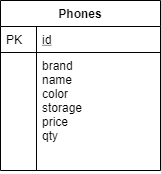
\includegraphics{dbschema.png}}
  \caption{Database schema}
\end{figure}

\subsection{Python modules}
\begin{itemize}
  \item \texttt{tkinter}: The core graphical user interface functions in the application
  \item \texttt{tkinter.ttk}: Used for Treeview, while editing, showing, deleting the phones entries
\end{itemize}

\subsection{Classes structure}
A main point of the interaction between the users and the application is the user interface. Therefore, designing windows that are simple to use is an important task for the project. The windowing subsystem manages a few functional windows, each in turn manages its own work. Functions support each other in order for the system to run. 

The classes are decoupled, meaning if one of them does not work (because of anything), the system can still normally function.

\begin{itemize}
  \item Sidebar (windows/sidebar.py)
    \begin{itemize}
      \item Placed on the left column of the application
      \item Contains Add, Edit, Show, Delete, Import, and Quit buttons
    \end{itemize}
  \item WinLog (windows/log.py)
    \begin{itemize}
      \item Placed under the functional window area, on the right column of the application
      \item Used for writing running status. The mechanism is written below.
    \end{itemize}
  \item WinManager (windows/manager.py)
    \begin{itemize}
      \item Is not displayed
      \item Used for managing the current active functional window and switching windows
    \end{itemize}
  \item Functional windows
    \begin{itemize}
      \item WinEdit (windows/edit.py)
      \item WinShow (windows/show.py)
      \item WinDelete (windows/delete.py)
      \item WinStatus (windows/status.py)
    \end{itemize}
  \item Models
    \begin{itemize}
      \item Database (models/database.py): For database specific controls
      \item Mobilephone (models/mobilephone.py): For mobilephone details and database interaction
    \end{itemize}
\end{itemize}

\subsection{I/O structure}
\begin{itemize}
  \item Input fields are on specific functional window
  \item Output are updated to the log bar through \texttt{WinLog.update\_log()} and saved to database when necessary
\end{itemize}

\subsection{UI structure}
\begin{itemize}
  \item WinManager (windows/manager.py)
    \begin{itemize}
      \item Maintain active functional window
      \item Handle different functional window switching when sidebar buttons are pressed
      \item Manage the geometry of the windows (pack, grid, etc.)
    \end{itemize}
  \item main.py
    \begin{itemize}
      \item Initialize Sidebar, WinLog
      \item Put WinStatus as current active functional window via WinManager
      \item Manage the geometry of the base frames (where to put the windows)
    \end{itemize}
\end{itemize}

\subsection{Sample data}
\begin{itemize}
  \item In the file sample.sql
  \item Use for initialize sample data for testing
\end{itemize}

\newpage

\section{Test the application}
\subsection{First impression}
User can launch the application via \verb|python main.py|. At first glance, the user can see our app with many sidebar buttons, on the left of the app, showing that the usage is trivial. It is just clicking buttons. The log window is placed closed to the bottom, and to the right of the sidebar. The status is displayed in the functional area.
\vspace{4cm}
\begin{figure}[H]
  \centerline{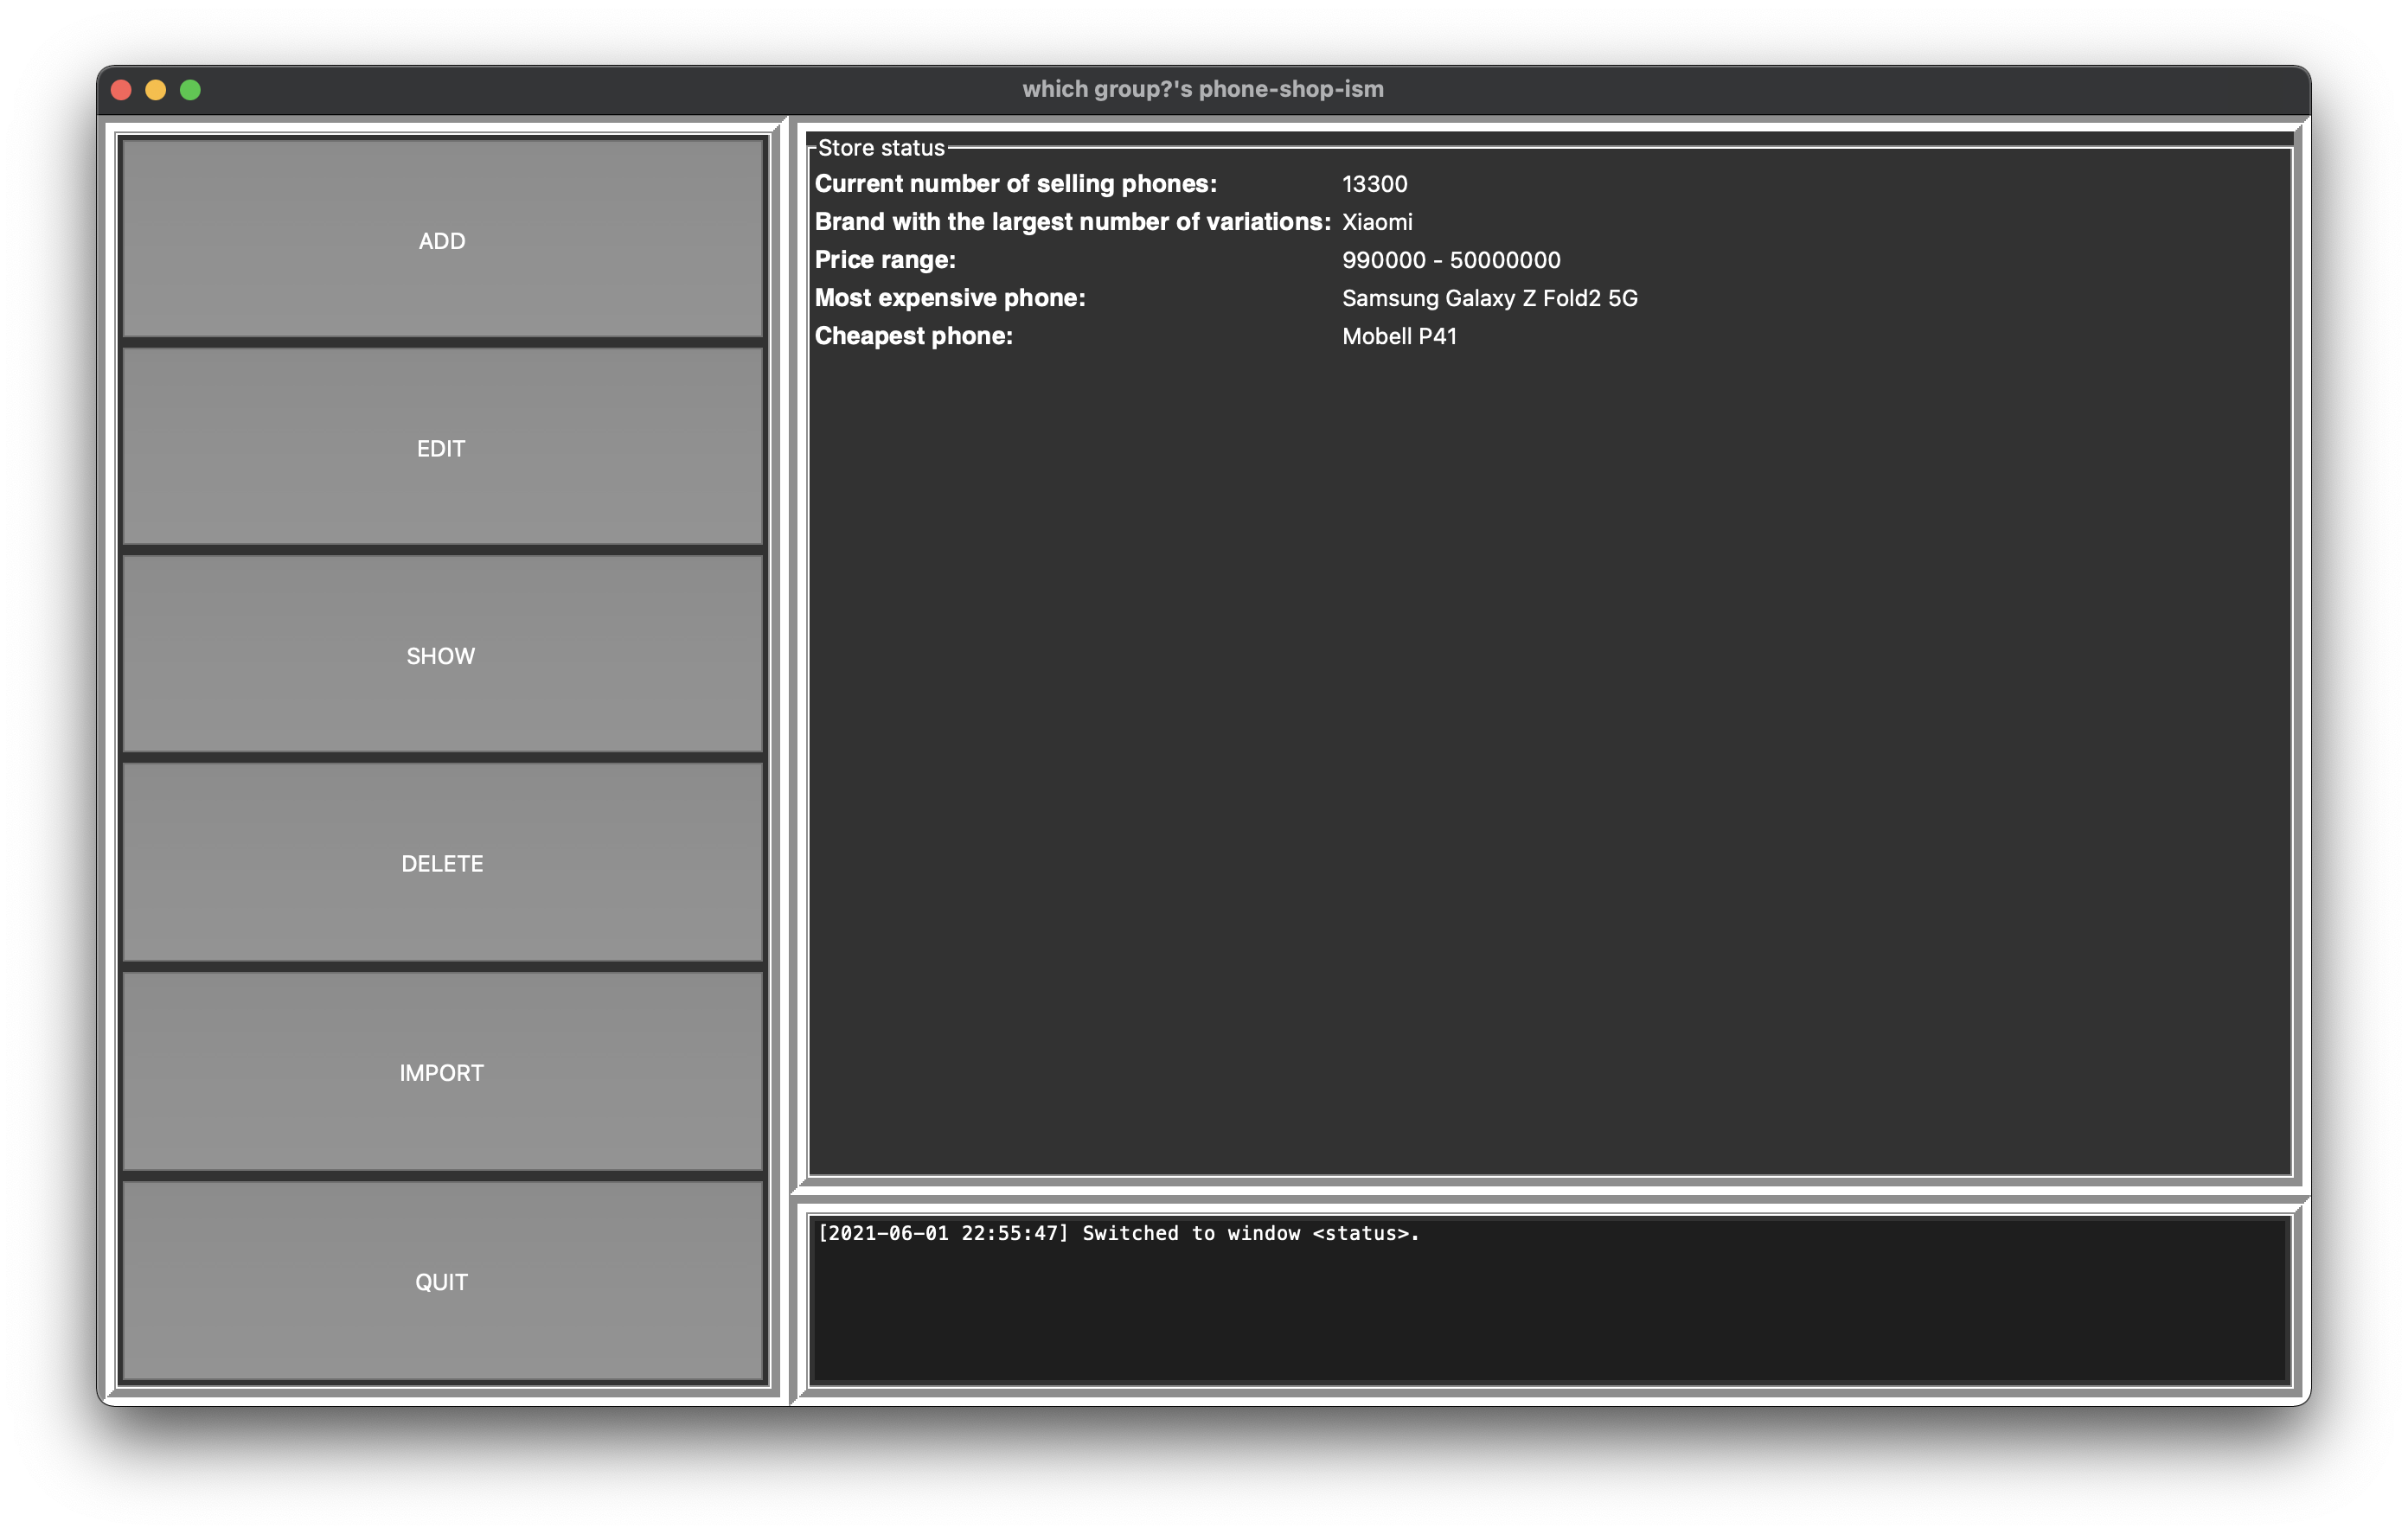
\includegraphics[scale=0.35]{launch-time.png}}
  \caption{Launch interface}
\end{figure}

\newpage

\subsection{The sidebar buttons}
\subsubsection{Add button}
Clicking this button will display a menu at the top left corner of the functional area. The user can fill the values in each entry. The "Add" button in this menu will execute database update if all fields are valid (using simple validation). If some of the fields are invalid, the errors are logged to the log window. If the user wish to reset the fields, they can just click the "Clear" button, which will reset all fields to blank.
\begin{figure}[H]
  \centerline{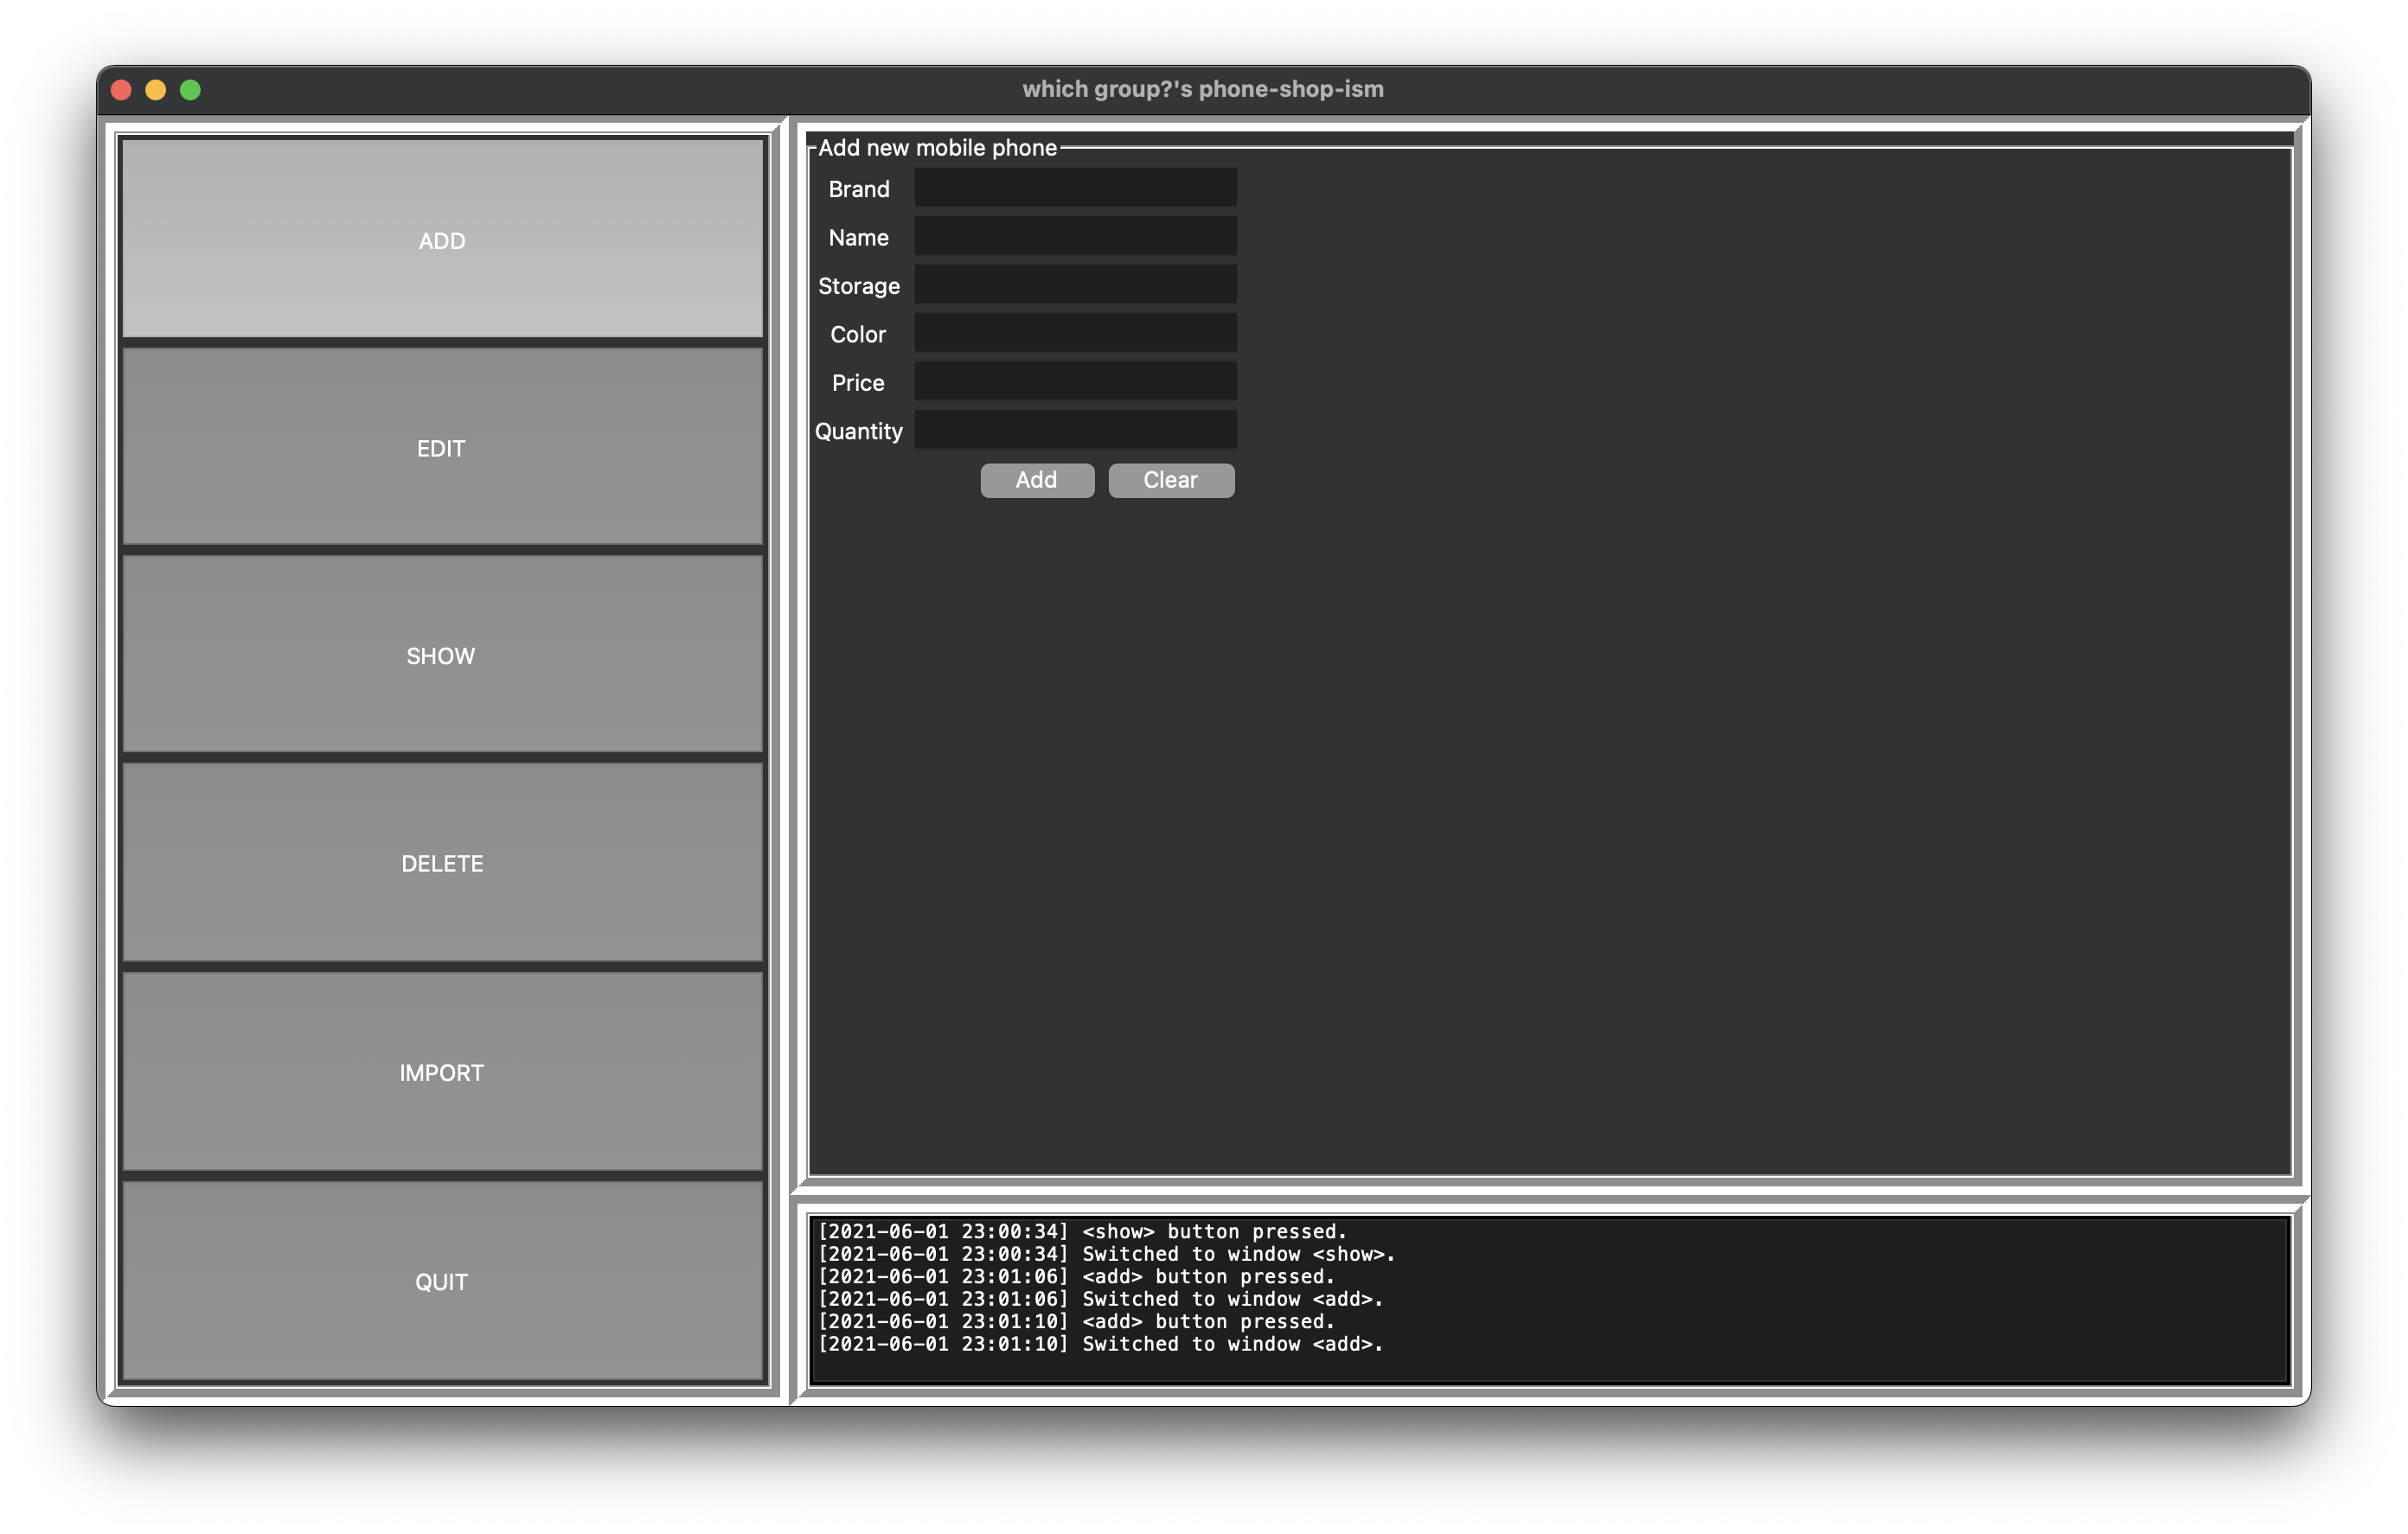
\includegraphics[scale=0.35]{add-clicked.png}}
  \caption{Add button interface}
\end{figure}

\subsubsection{Edit button}
Our application enable the user to edit every information of the phone as we mentioned before by clicking this button, which will then show the user the list of all phones. Clicking on any of these entries display the edit menu. The "Update" button will execute database update if all fields are valid, errors are logged to the log window instead. The "Clear" button resets the fields to original values.
\begin{figure}[H]
  \centerline{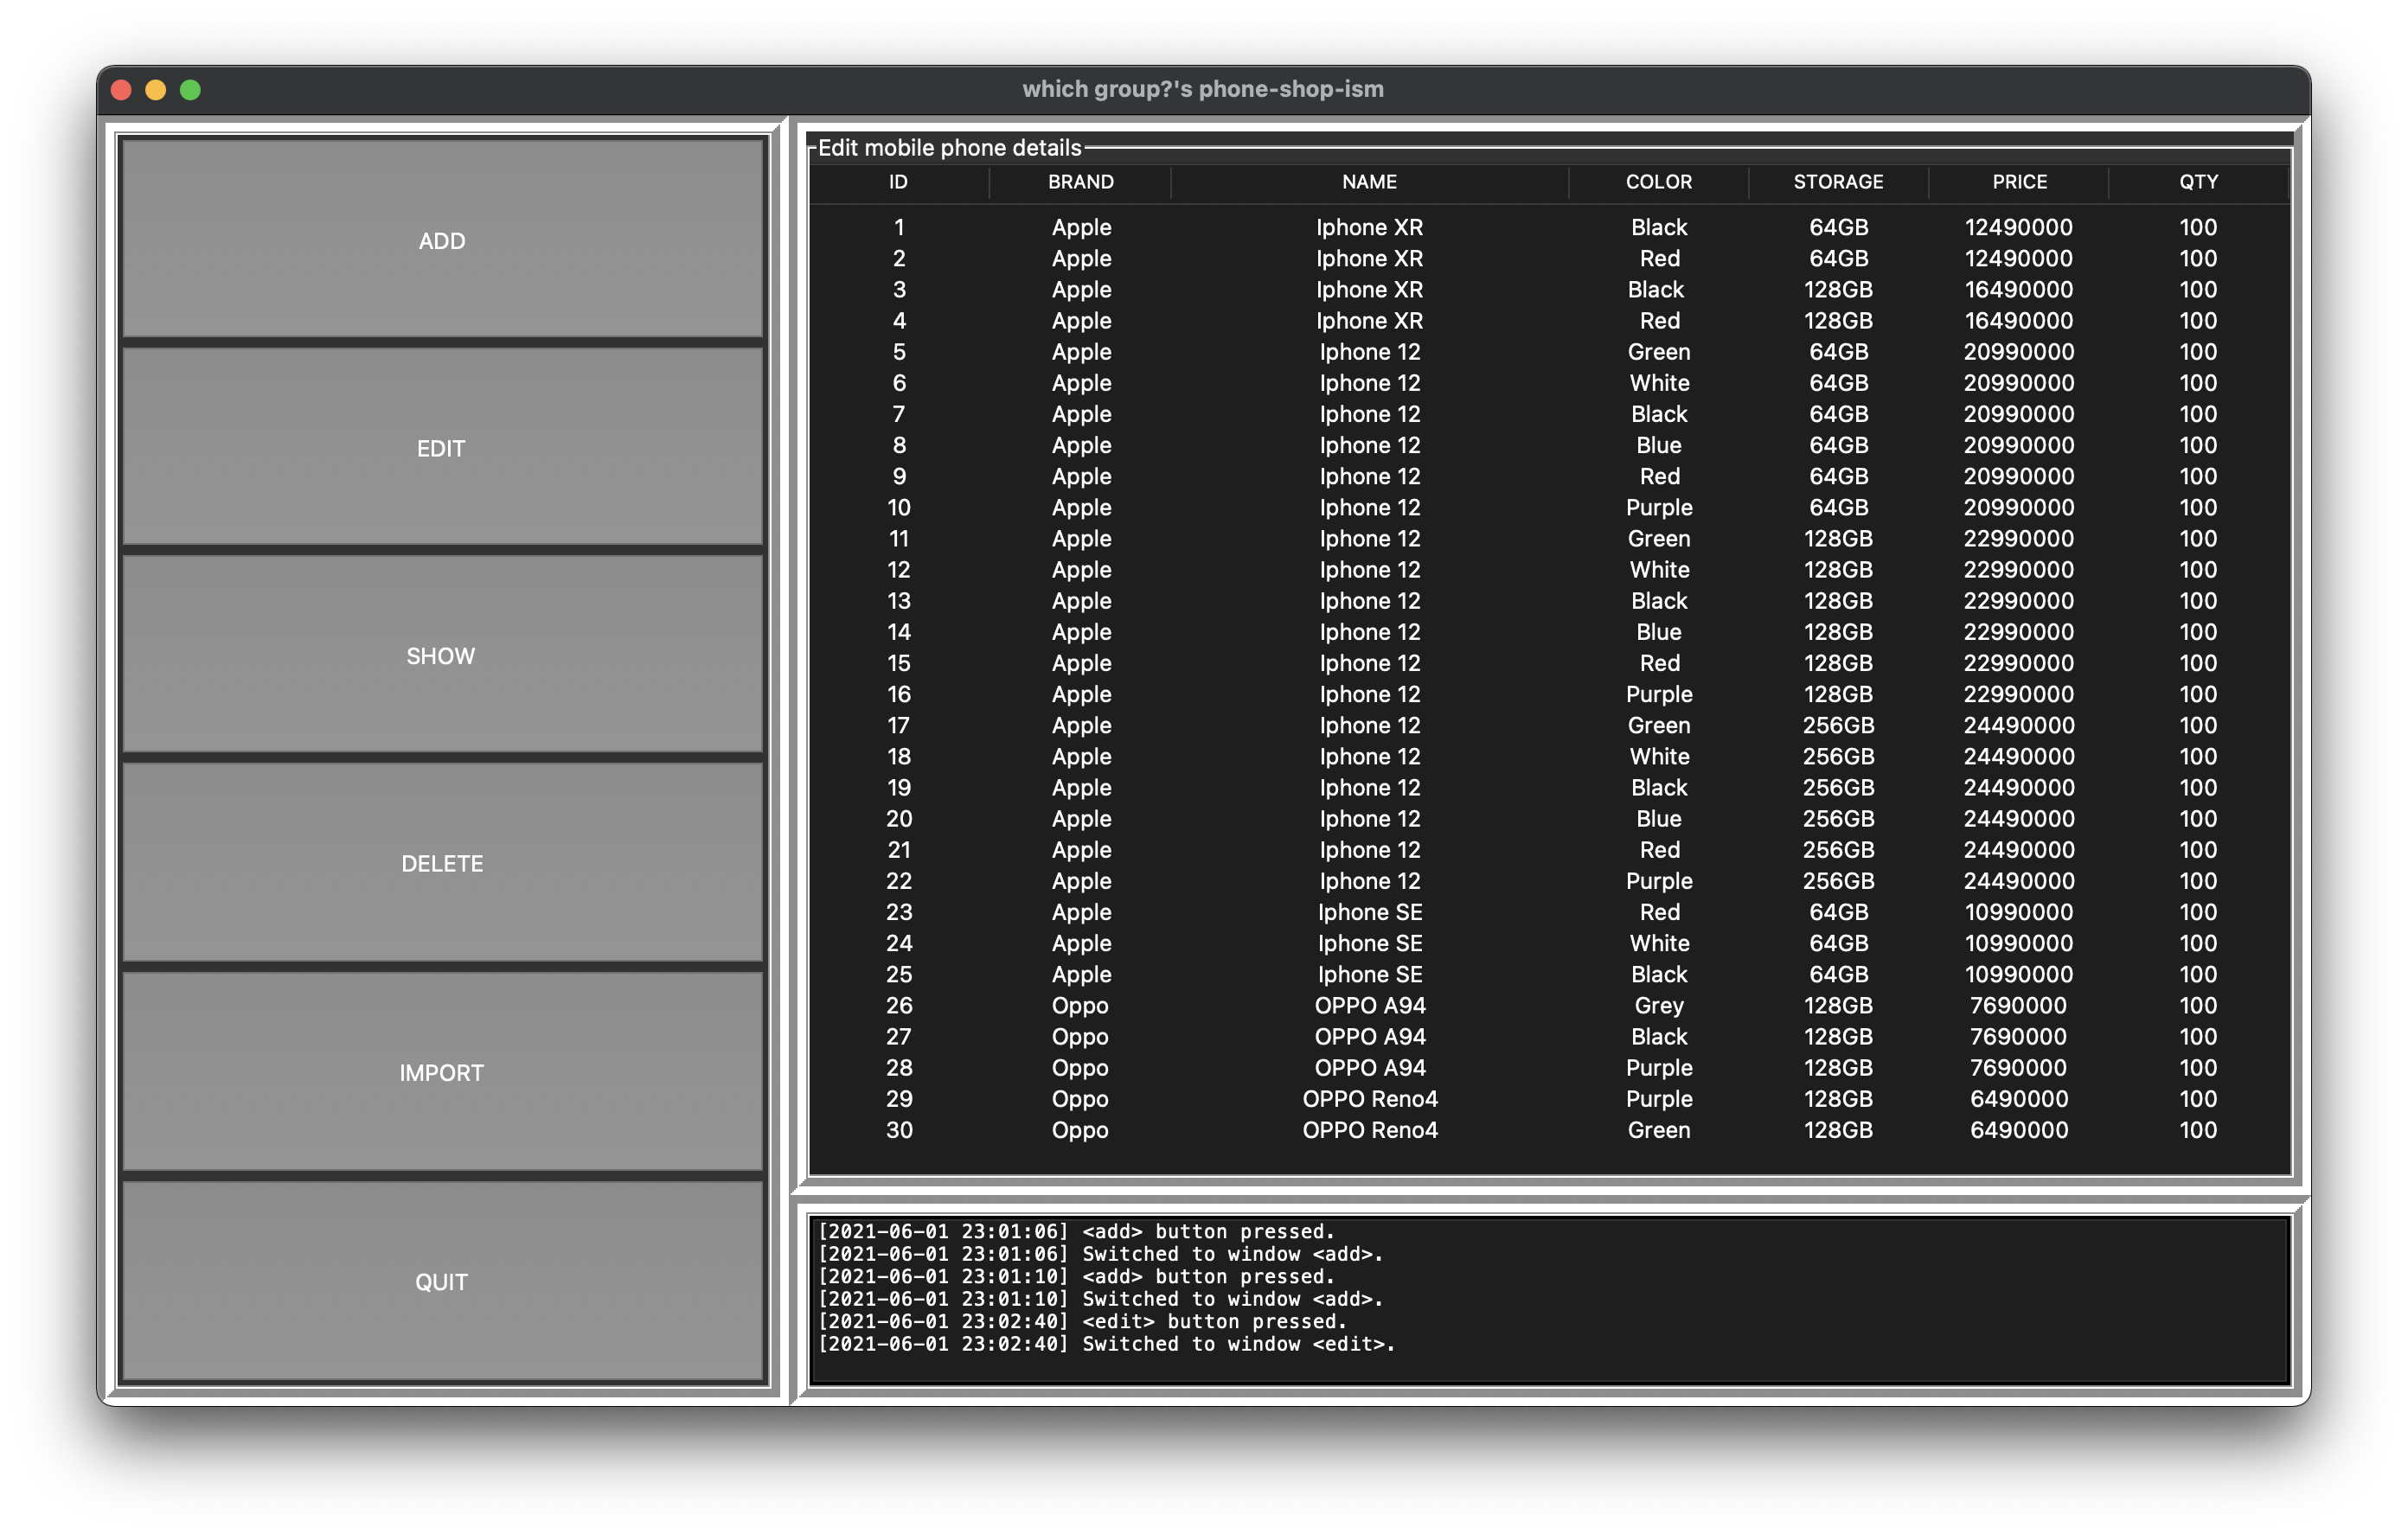
\includegraphics[scale=0.35]{edit-clicked.png}}
  \caption{Edit button interface}
\end{figure}

\begin{figure}[H]
  \centerline{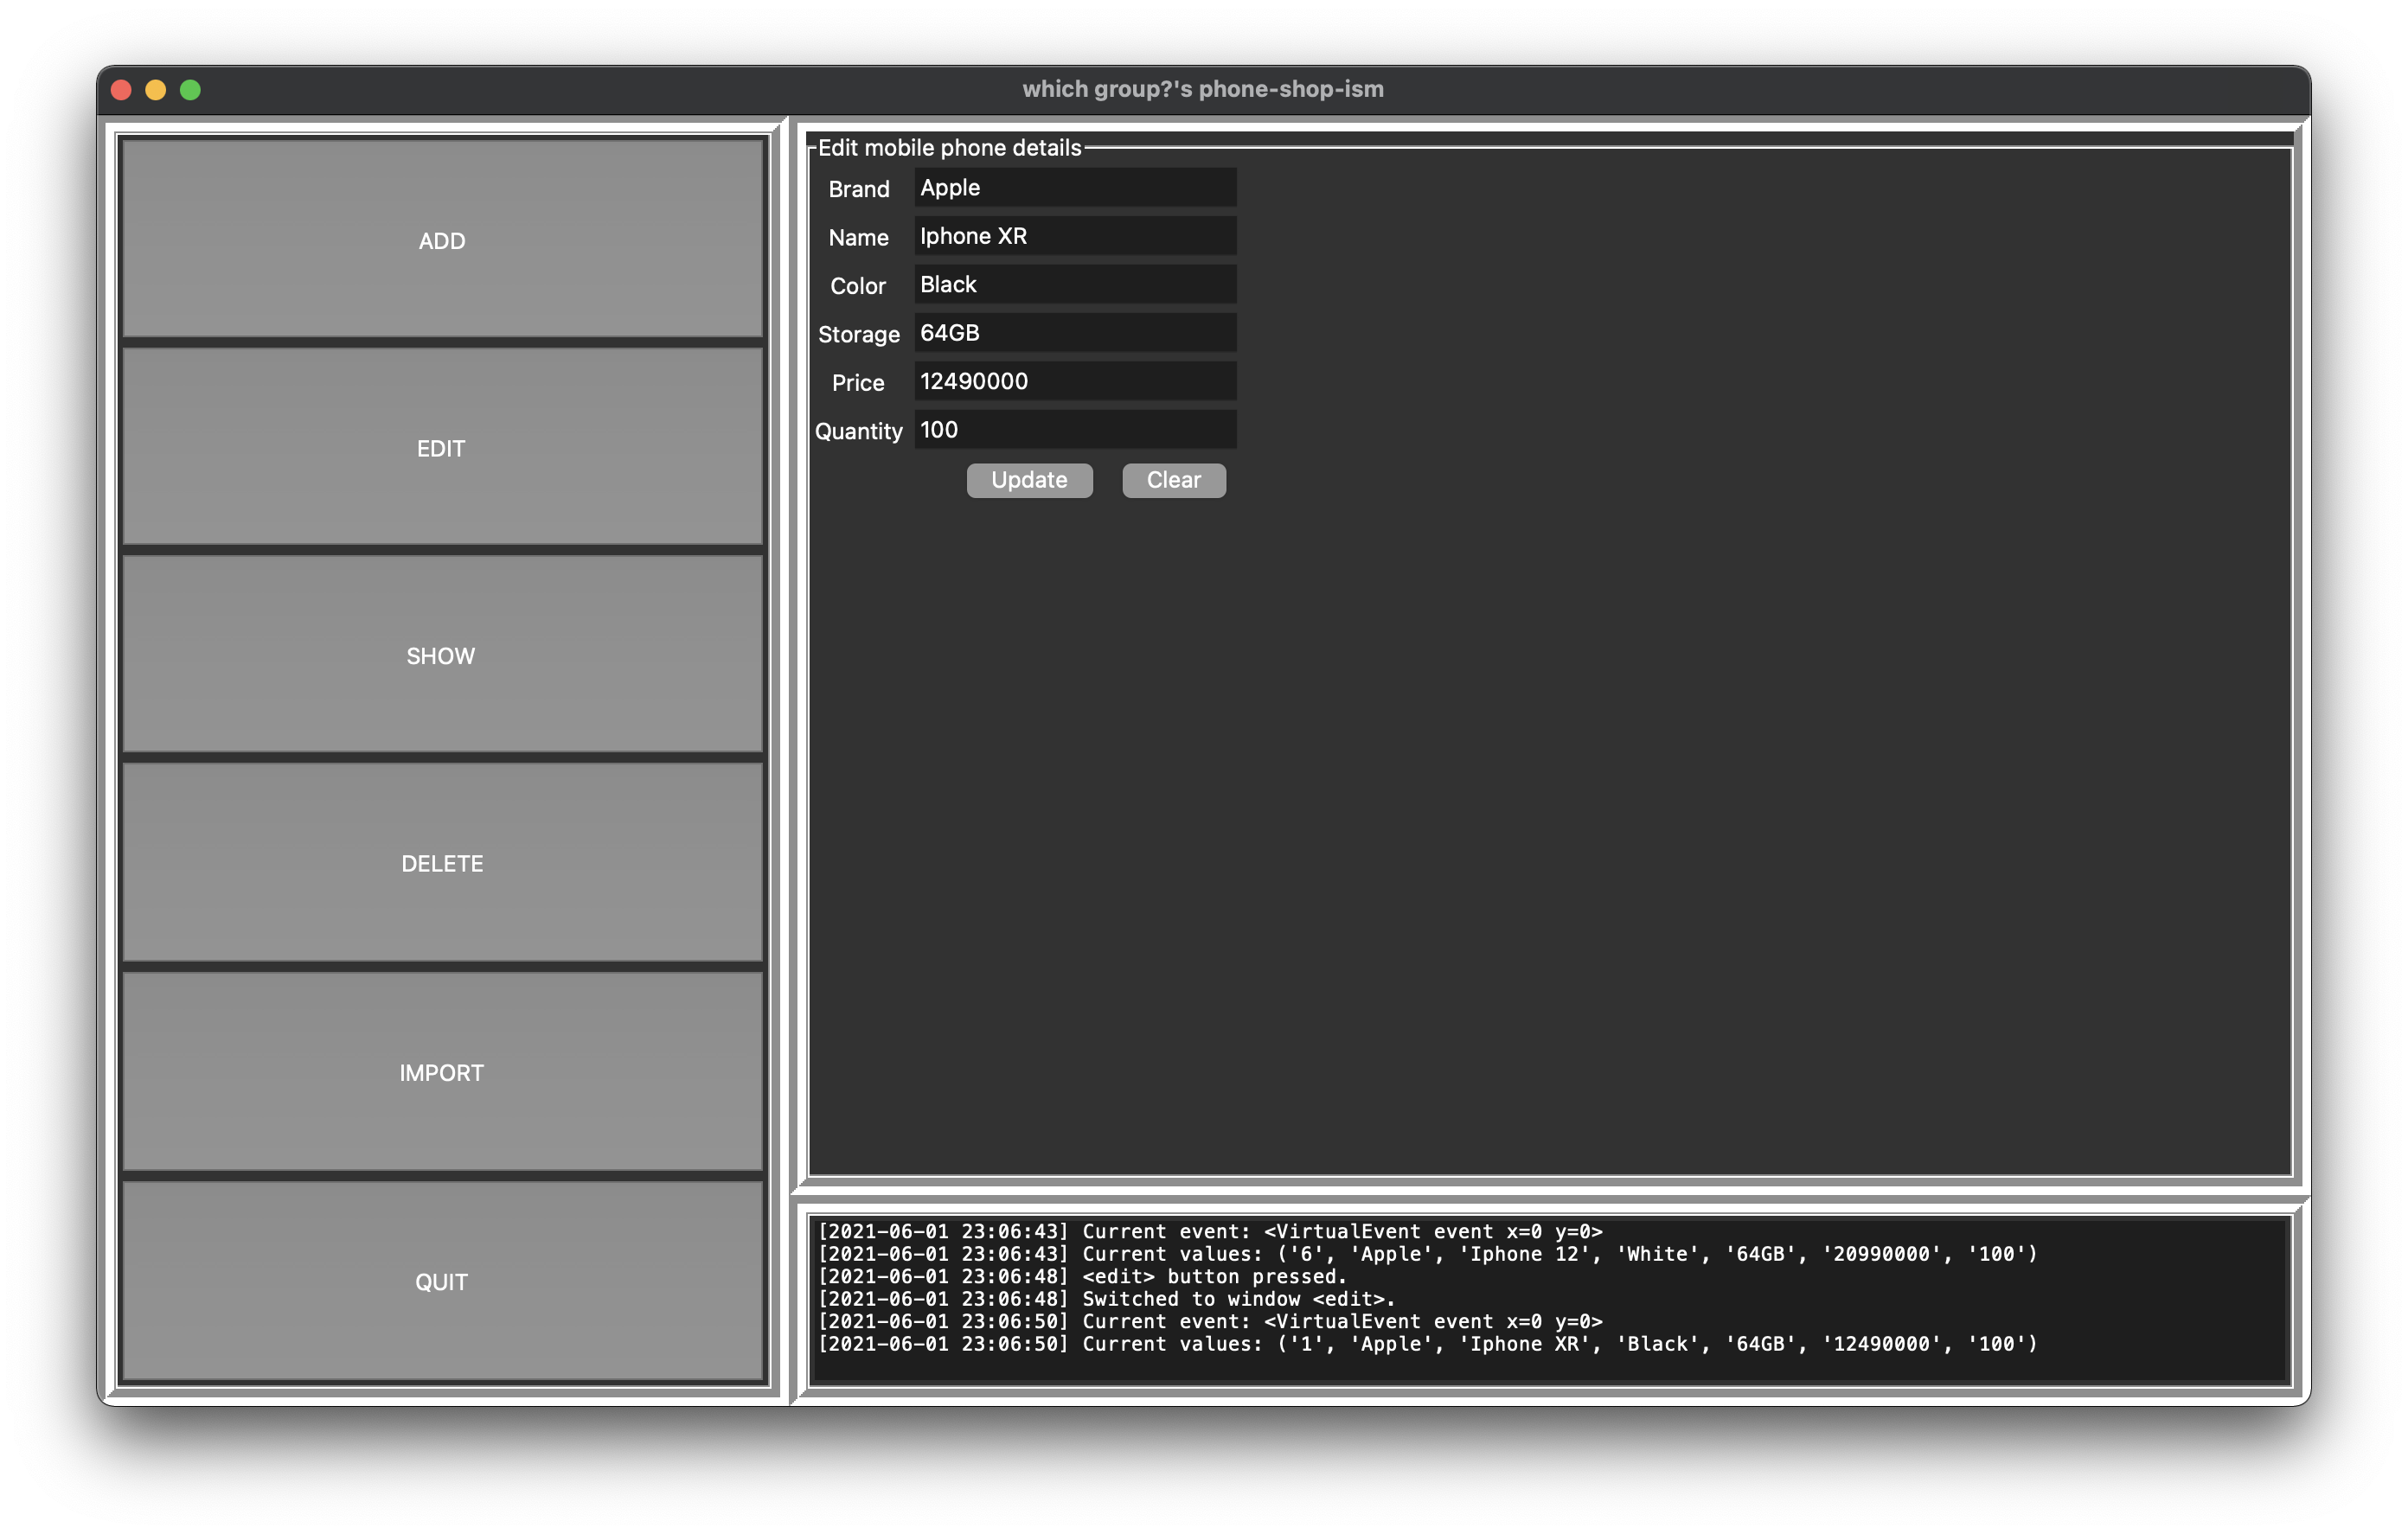
\includegraphics[scale=0.35]{edit-entry-clicked.png}}
  \caption{Edit phone details}
\end{figure}

\subsubsection{Show button}
If the user click this button, the functional area will display the list of all phones.
\vspace{4cm}
\begin{figure}[H]
  \centerline{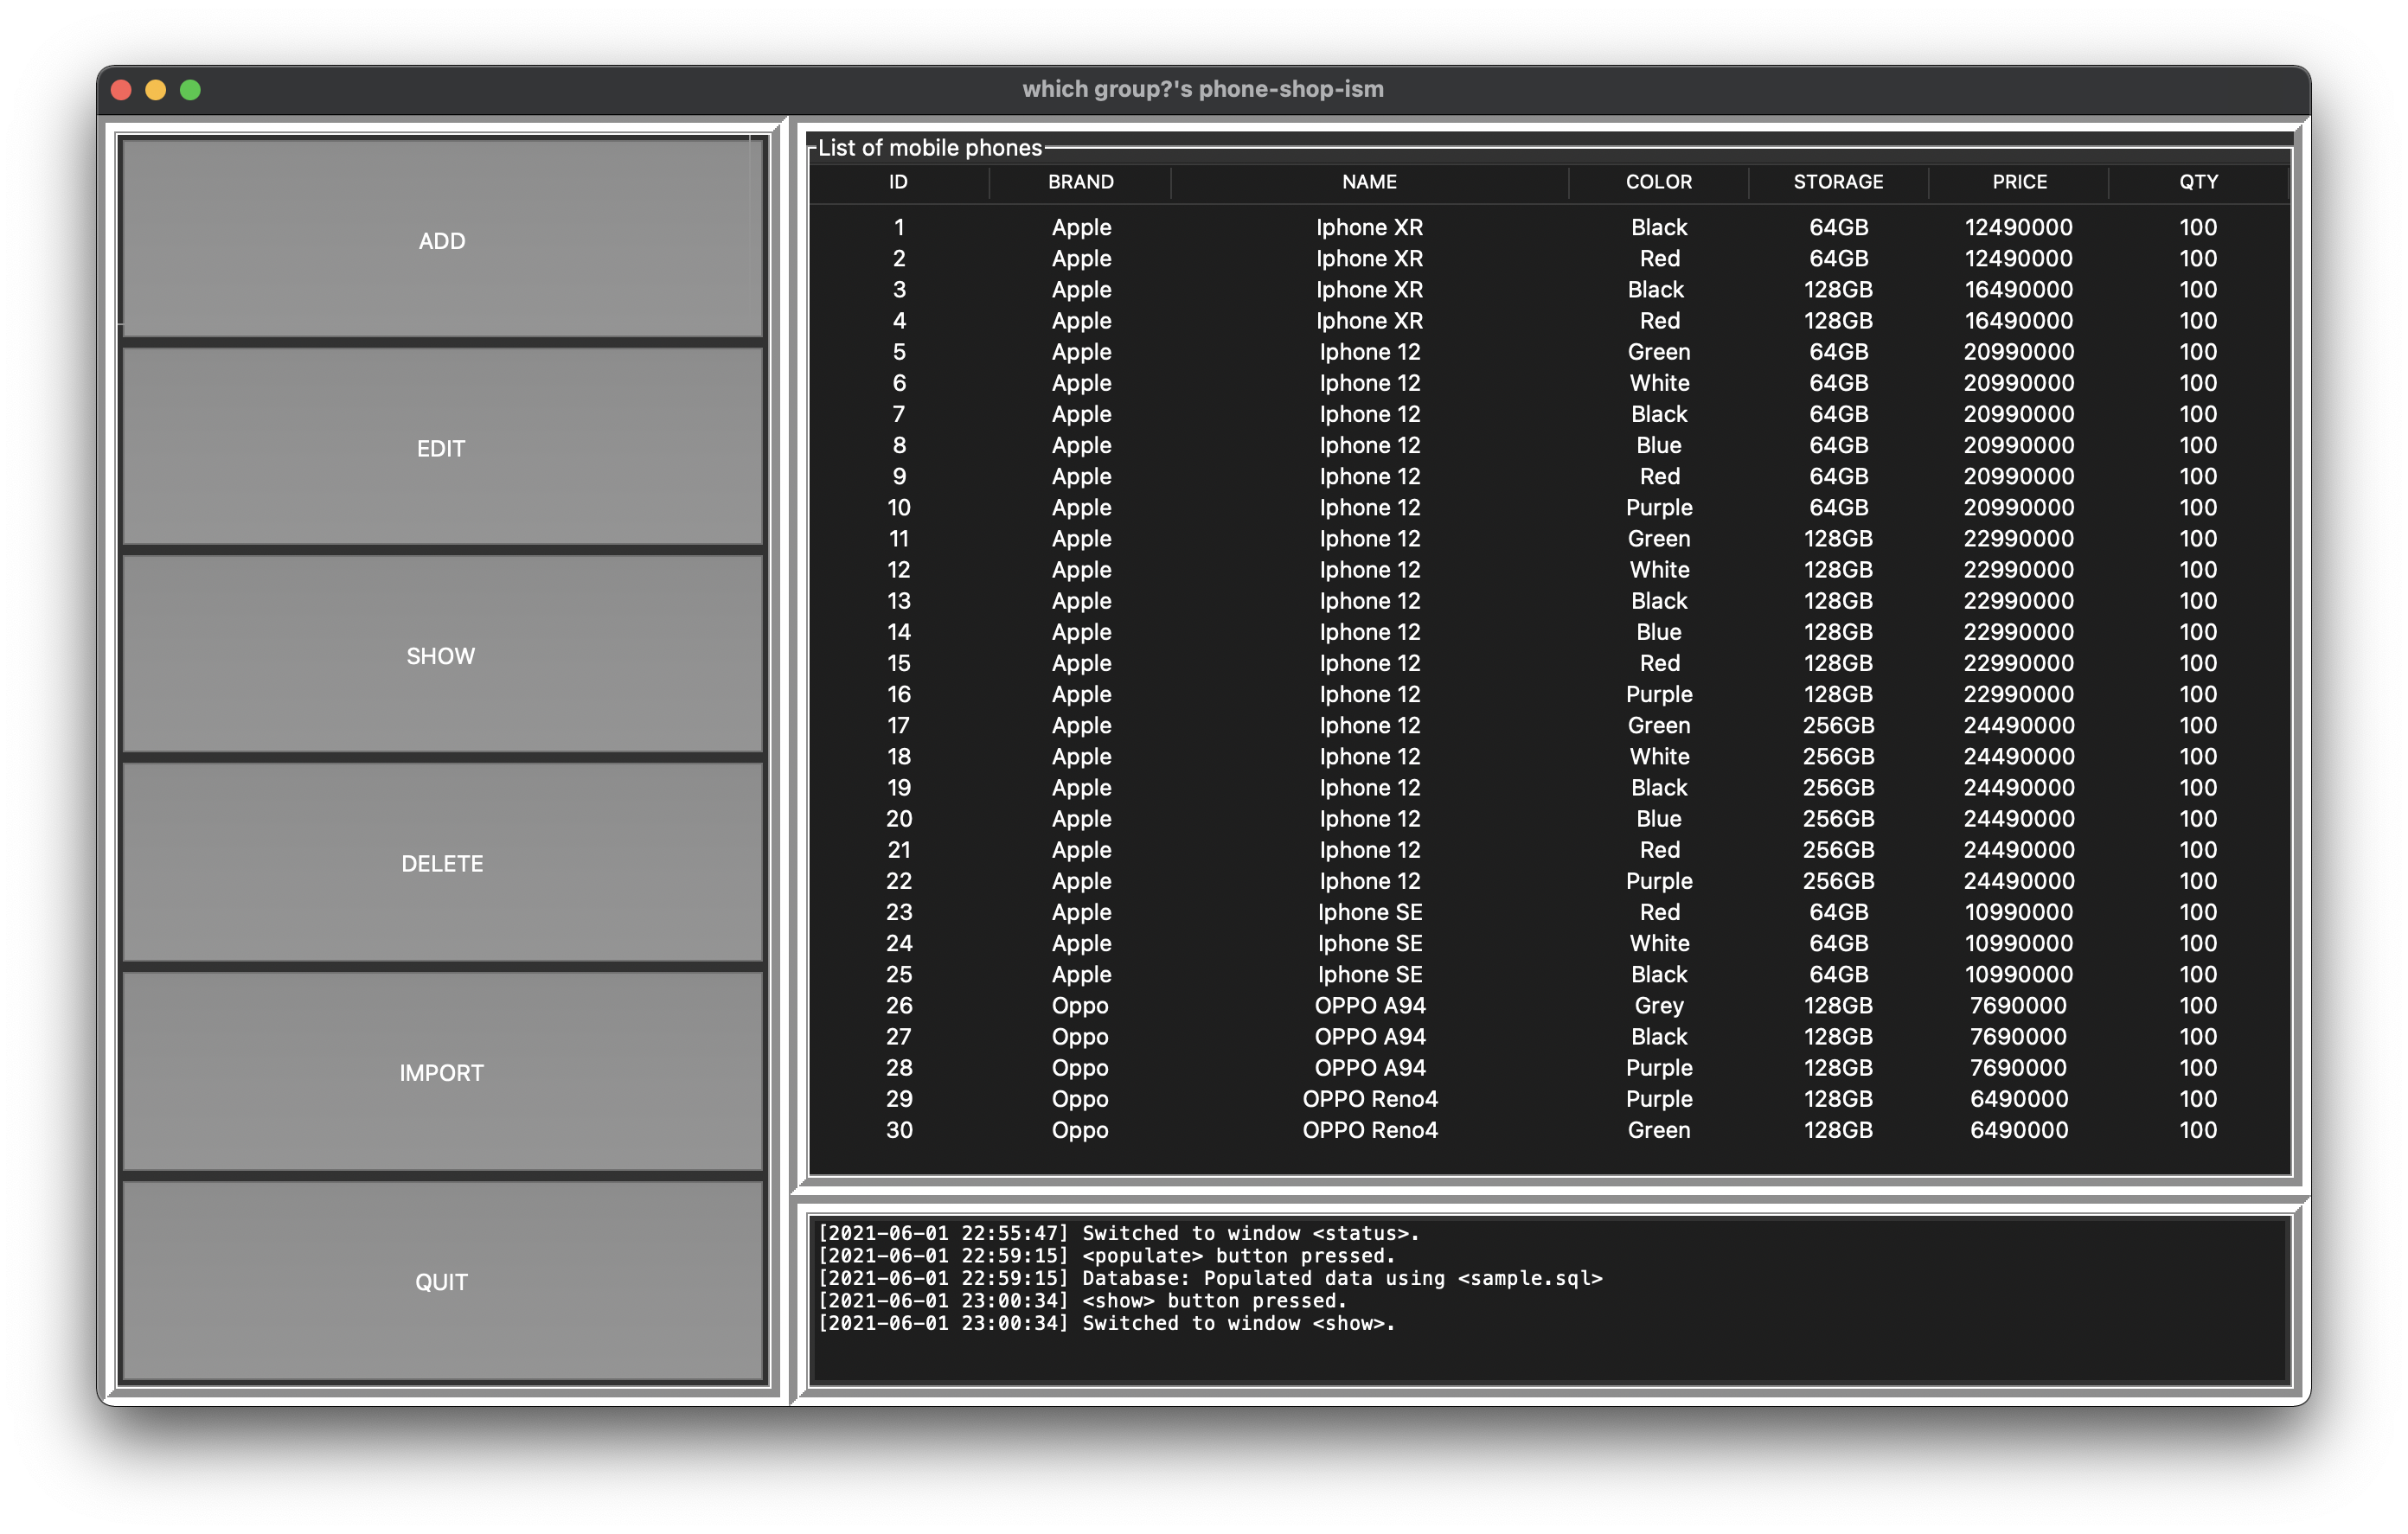
\includegraphics[scale=0.35]{show-clicked.png}}
  \caption{Show interface}
\end{figure}

\newpage

\subsubsection{Delete button}
When this button is clicked, the label becomes "Delete mobile phones". Click on any line pops up a message to confirm the delete action to the specific entry. "Yes" will execute database update to delete the row, "No" will leave the database intact.
\begin{figure}[H]
  \centerline{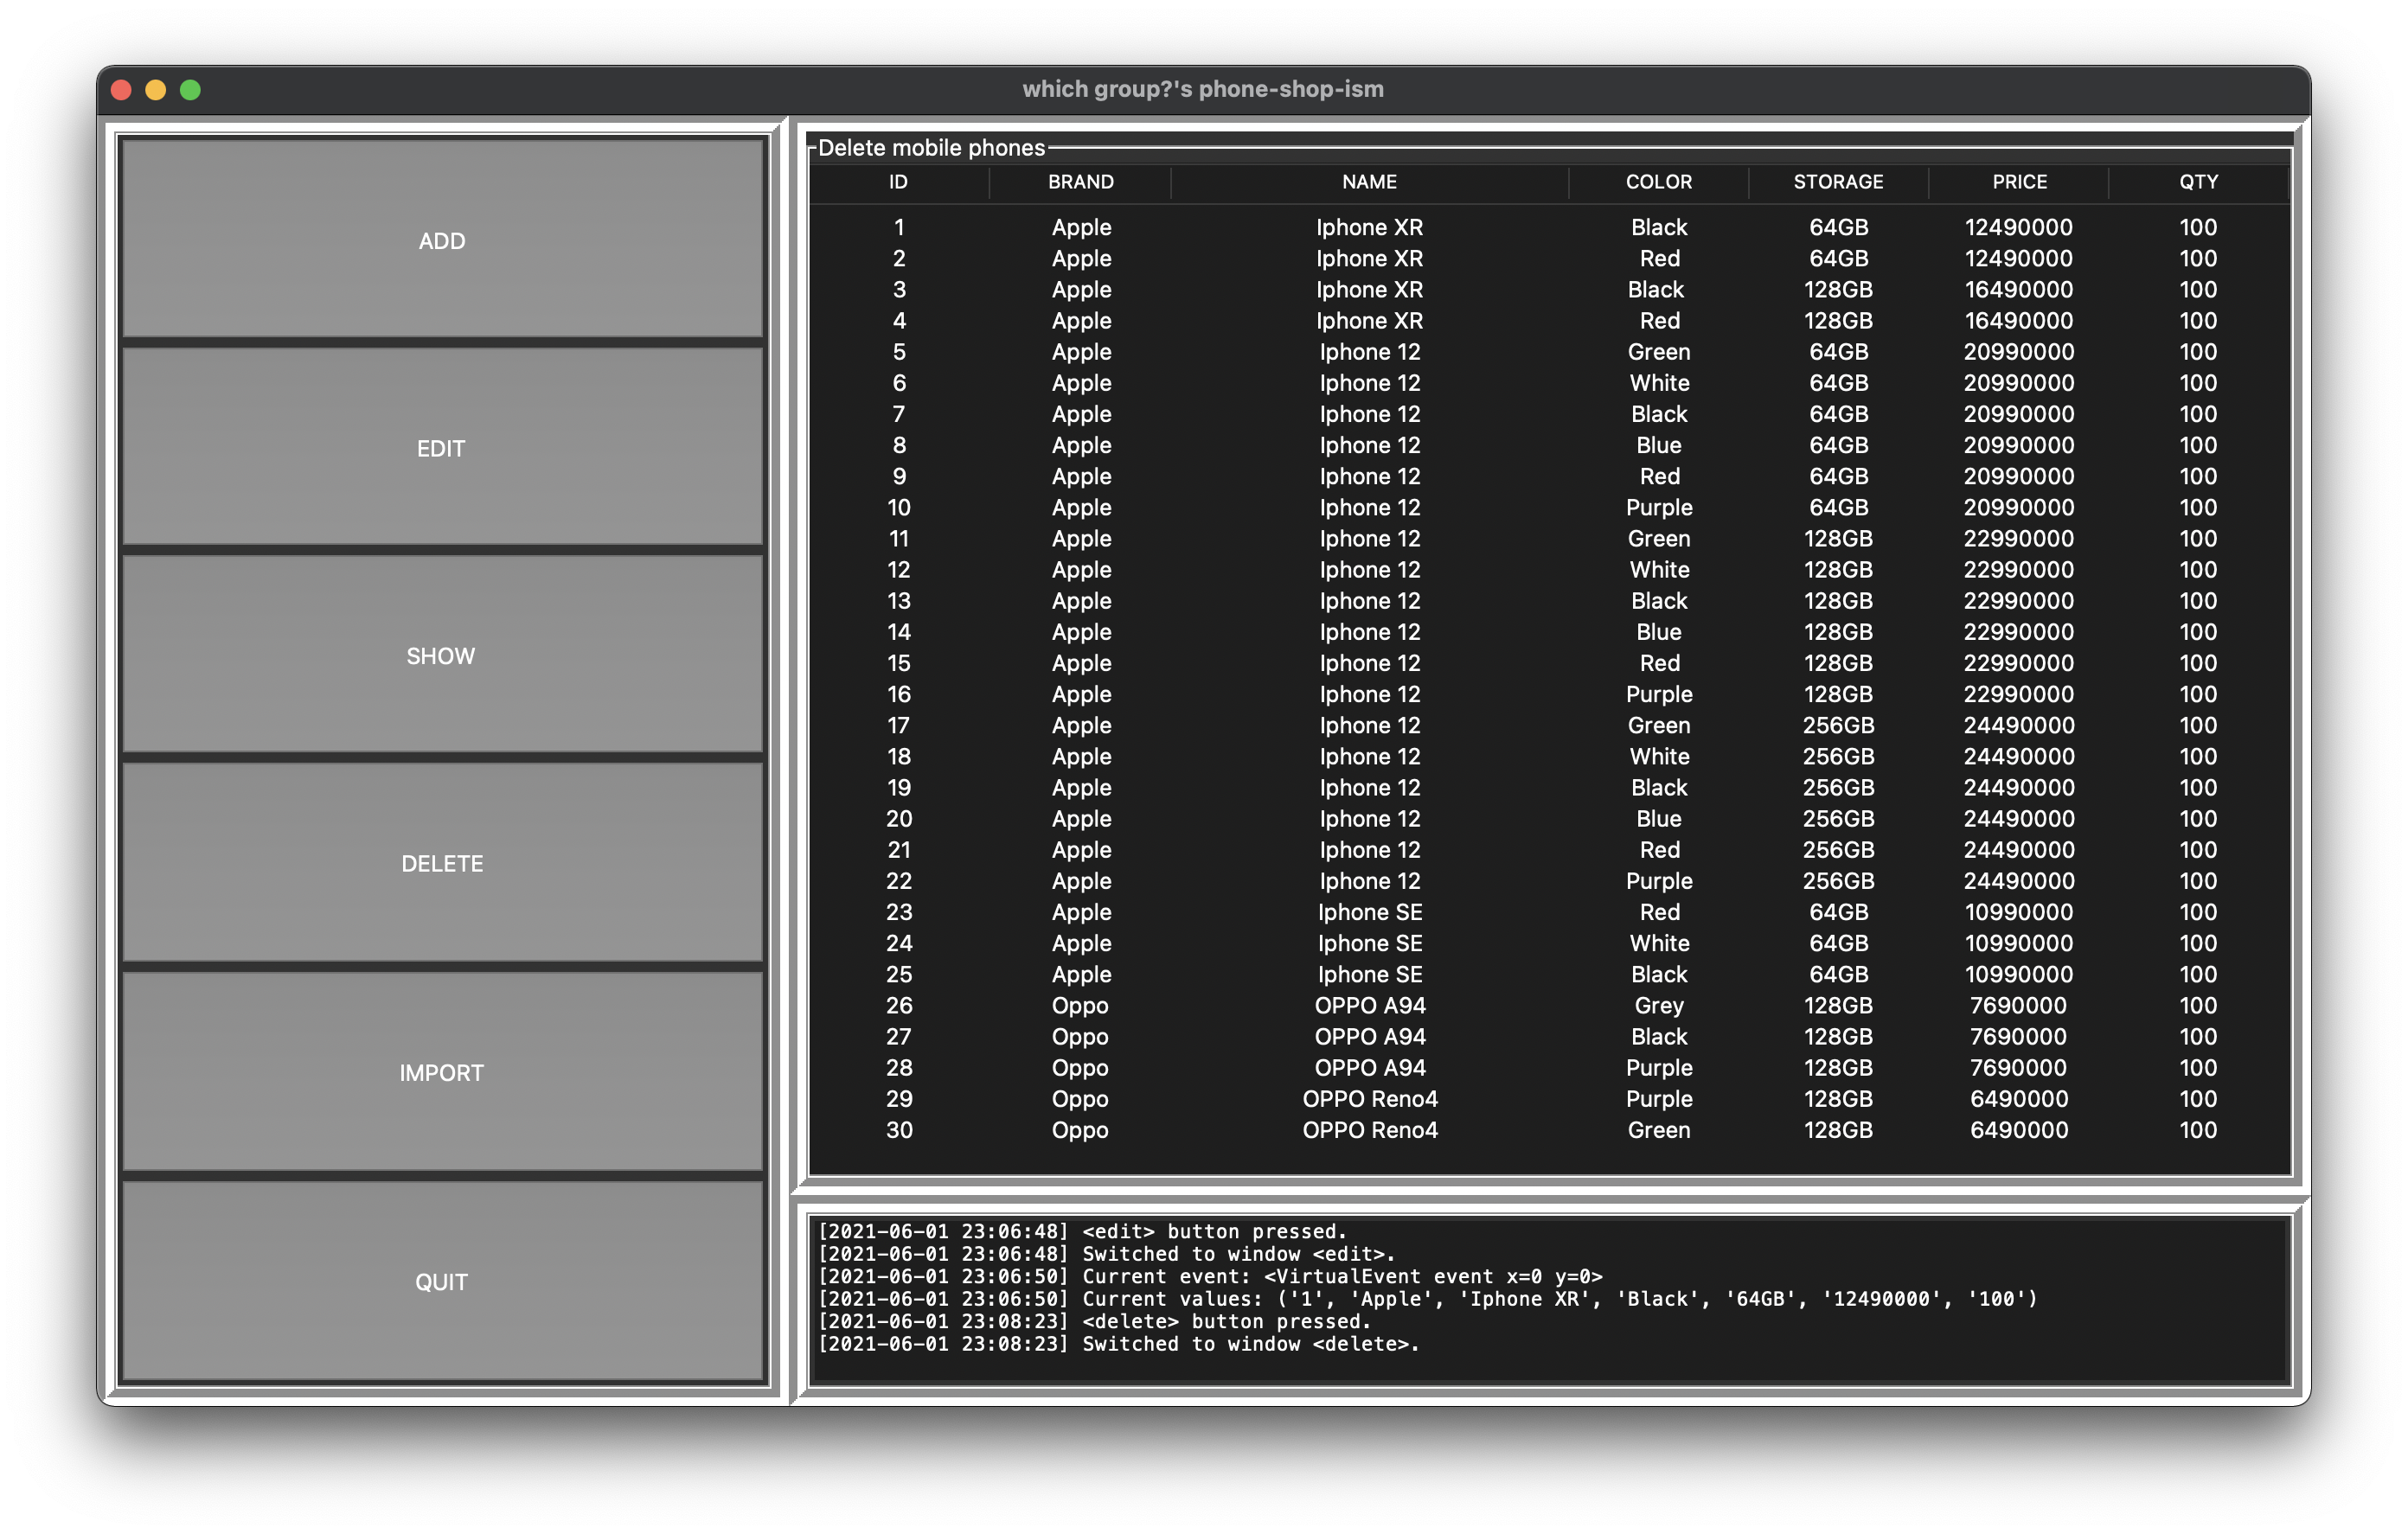
\includegraphics[scale=0.35]{delete-clicked.png}}
  \caption{Delete interface}
\end{figure}

\begin{figure}[H]
  \centerline{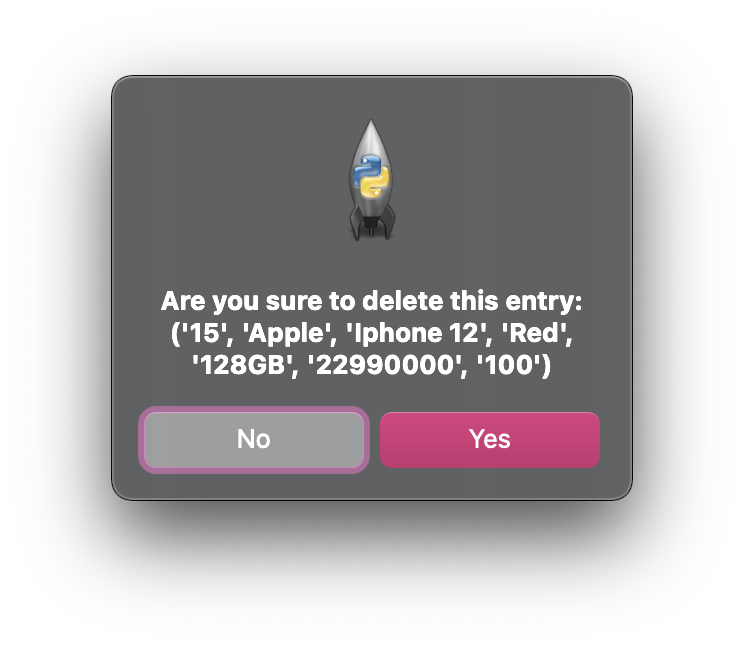
\includegraphics[scale=0.5]{delete-entry-clicked.png}}
  \caption{Delete popup}
\end{figure}
    
\subsubsection{Quit button}
The "quit" button will close the app. Prior to closing, it disconnects the database and destroy the windows.

\newpage

\section{Comments}
\subsection{What we have done}
\begin{itemize}
  \item A working information manager with minimal set of features, that can be used as a base for developing further
  \item Minimal database design (perhaps mediocre as well)
  \item Minimal user interface
  \item And the application was intended for use by managers
\end{itemize}

\subsection{What could be improved}
\begin{itemize}
  \item Split the single database table into many, or use other attributes and assumptions
  \item Fix the space taken by the sidebar to a reasonable size
\end{itemize}

\subsection{What we could have done}
\begin{itemize}
  \item A login subsystem. In fact, the code for securely hashing passwords and checking them is ready, but the extra time to insert a new database table and testing Tkinter UI will be well over the deadline.
  \item Buttons and windows colors.
  \item Reports generation. The idea and Python code was ready, but like with the login feature, we could not allocate enough time for it.
  \item A customer view so that sell, sale off, and many store features may be implemented.
\end{itemize}

\subsection{Current detected errors}
\begin{itemize}
  \item When switching windows, the labels of the new windows are sometimes not updated. This issue persists on macOS but not on Windows.
  \item The database needed to be there before launching the application, because the WinStatus class will need it. This renders the Import button useless, but it could be fixed by introducing a "information unavailable" view to the status window.
\end{itemize}

\section{Conclusion}
We have spent quite a huge amount of time to complete this project, and while it is not perfect, the application can still work, if the users are patient enough. Our application missed some common features, and that should have been implemented, but our lack of time and experience were the main reason why we could not make it in time. We consider it our success because the crying weeks before the application can run were worth it.

\end{document}
